\documentclass[conference,9pt]{IEEEtran}
\usepackage{xcolor}
\usepackage{cite}
\usepackage{epsfig}
\usepackage{amssymb}
\usepackage{amsmath}
\usepackage{graphicx}
\graphicspath{ {../} }

\begin{document}
%\tableofcontents
%\textheight=22.6cm
%
% paper title
\title{Practical 1B}

% author names and affiliations
\author{
	\IEEEauthorblockN{Albert Acebron}
	\IEEEauthorblockA{NIU: 1458626}
}


% make the title area
\maketitle
\begin{abstract}
	In this practical we'll touch on removing the doppler effect, decimating signals and detecting unknown symbols
\end{abstract}

%----------------------------------------------------------------
% SECTION #1 
\section{Introduction}
This practical will be focused on the second half of the DSP pipeline we're working on, which handles the signal after it has been digitized and the gaussian noise has been removed.

More concretely, we will be decoding the signal down to the symbols that were originally sent by removing any interferences and extracting information from it.

\section{Questions}
\subsection{Question 1}
The number of samples per symbol can be calculated as:
$$N_{ss}=F_s \cdot T_{sym}=20\cdot10^6 \cdot 10^{-6} = 20$$

\subsection{Question 2}
We will apply the method described in question 3 of the previous lab to normalize the filter:

\begin{verbatim}
filter = pam_sqrrc(20, 20, 0.35, 1);
energy = sum(filter.^2)
filter = filter/sqrt(energy);
\end{verbatim}

\subsection{Question 3}
This is achieved by applying the energy calculation performed in the previous practical to the absolute values ($\sqrt{real^2+imag^2}$) of the complex numbers obtained from the convolution.

\begin{verbatim}
output = add(RxSignal, filter)
avg_energy = sum(imag(output).^2 
+ real(output).^2)/length(output)
\end{verbatim}

Which results in an average energy of 0.96. We've also checked the output comparing it with the result of "conv(RxSignal, output)" and the length is the same.

\subsection{Question 4}
Given that the change caused by the doppler effect just translates into specific multipliers that are applied to each output value, these can be cancelled by multiplying every value by it's corresponding multiplicative inverse, that is:
$$a\cdot e^{jwn} \cdot e^{-jwn} = a$$

We can apply this to $y$ to remove the dopler effect:
$$y_{clean}(x)=y_{doppler}(x)\cdot e^{-jwn}$$

And given that $F_d=50$, we know that $w=2\pi f=100\pi \dfrac{T_{sync}}{F_d}$ ($\dfrac{T_{sym}}{F_d}$) represents the time difference between samples), so we'll proceed to remove the effect with:
\begin{verbatim}
n=1:length(output)
no_doppler = output.*exp(-i*100*pi*n'*Tsym/Fd)
\end{verbatim}

\subsection{Question 5}
Given that we know that $N_{ss}=20$, it's trivial to see that this will be the period used for decimating, that is, between each value sampled there will be 19 that will be left out. The problem here is how to pick the offset from which to start sampling, as we have to take into account the changes applied in the previous steps, such as the convolution with a matched filter.

To do that let's remember that the matched filter is just a scaled version of the pulses that make up our input function, so if we plug that into the definition of convolution (using a single pulse for now):
$$y(t)=\sum_{k} p(k)p(t-k)$$
We see that what we have here are multiplications of two values, which, due to the growth curve of x*y, will grow much faster the higher the values are. Following that intuition it should be easy to see that the sum will be highest when the two functions match exactly.

Now if we consider that our pulse is symmetric against axis $x=\dfrac{N}{2}$ when $0\leq k\leq N$ we can conclude that the functions will match ($k=t-k$) when $t=N$.

This may have been a bit hand-wavy, but if we look at a set of SQRRC pulses (blue) and it's convolution with another SQRRC pulse we can verify that it holds true:
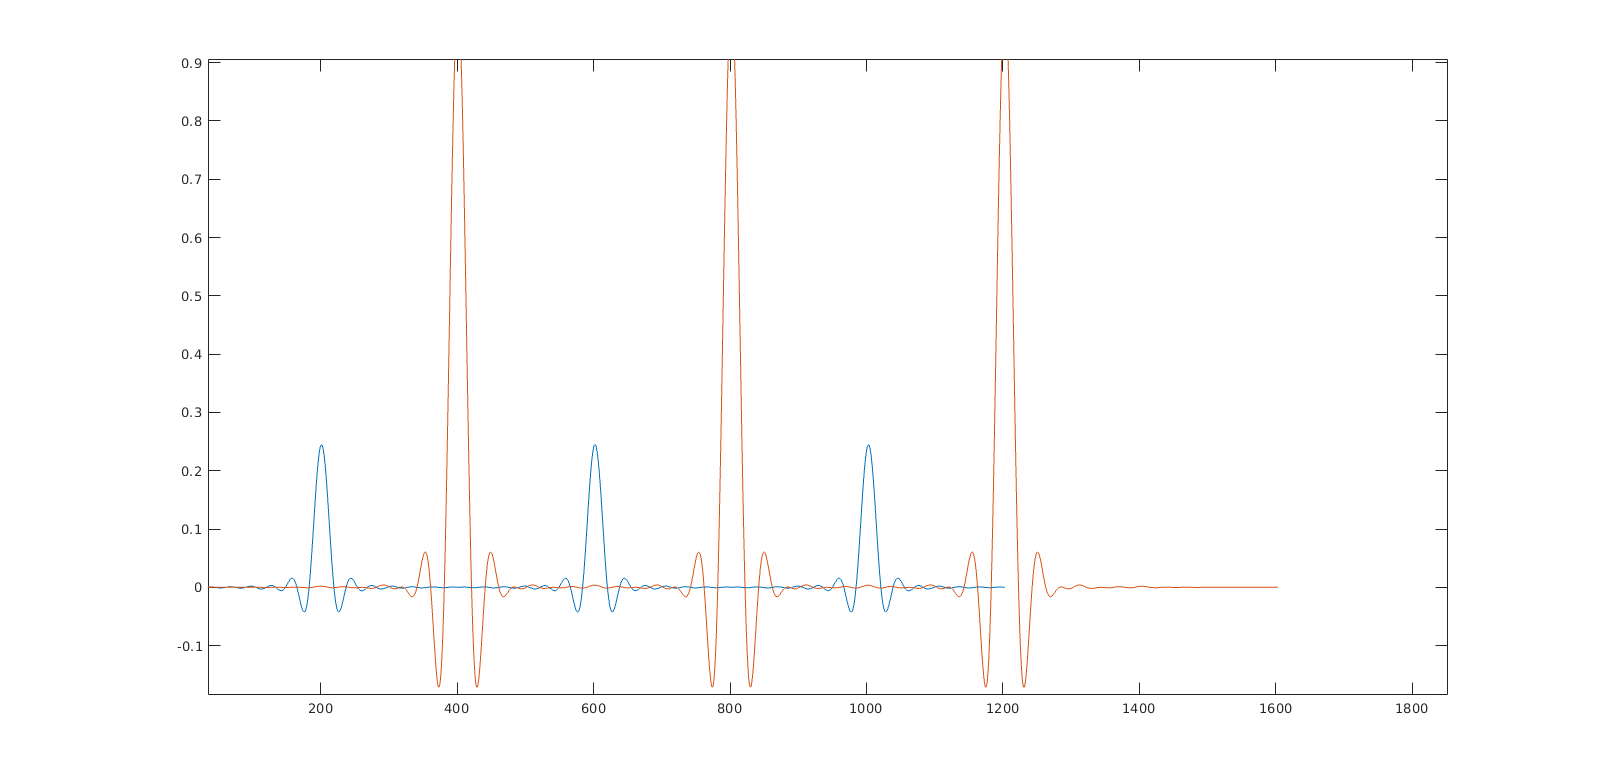
\includegraphics[scale=0.23]{convs}

In conclusion, we will decimate our signal at each 20th sample:
\begin{verbatim}
DecimatedSignal=no_doppler(20:20:end)
\end{verbatim}

\subsection{Question 6}
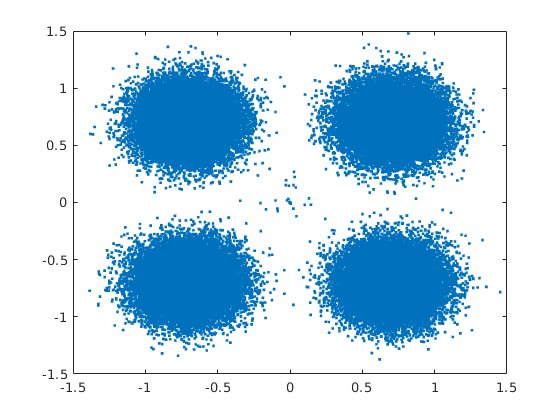
\includegraphics[scale=0.6]{res}
Looking at the graph we can clearly see that the constellation is a quaternary construction, where four symbols have been encoded into four different quadrants. The values at the center of the graph generally correspond to the ones at the start or end of the signal, as it's tails (~100 samples) have low amplitude.

\subsection{Question 7}
Given that we are dealing with a quaternary constellation, we know that ideally all points should be the same distance away from the center, so their energy will be also the same. Now, the average energy needs to be 1 and all samples should have the same energy so it's easy to see that the energy for each of them will need to be 1.

For that to happen, the imaginary ($img$) and real ($rea$) parts of symbol must meet the following identity:
$$img^2+rea^2=1$$

And due to how the points are ideally distributed, this can only happen  if:
$$abs(img)=abs(rea)=\sqrt{\dfrac{1}{2}}$$

So the symbols will all need to be of the form $(\pm\sqrt{\dfrac{1}{2}}, \pm\sqrt{\dfrac{1}{2}})$.

We can find the average energy of the constellation using the same method that we employed on question 3:
\begin{verbatim}
avg_cons_energy=sum(imag(DecimatedSignal).^2
  + real(DecimatedSignal).^2)/length(DecimatedSignal)
\end{verbatim}

Which resolves to 1.047, thus the average energy of the constellation is not strictly unitary but it is quite close to that.

\pagebreak
\subsection{Question 8}
Code:
\begin{verbatim}
function DetSymbols = symDetector(DecimatedSignal)

angles=atan2(imag(DecimatedSignal), real(DecimatedSignal));
DetSymbols=zeros(length(angles),1);
l=sqrt(1/2)

for i=1:length(angles)
    a=angles(i);
    if a>0
        if a<(pi/2)
            DetSymbols(i)=l+ l*j;
        else
            DetSymbols(i)=-l+ l*j;
        end
    else
        if a<(-pi/2)
            DetSymbols(i)=-l -l*j;
        else
            DetSymbols(i)=l -l*j;
        end
    end
end
\end{verbatim}

This results in the following graph when superimposed (detected values are red while sampled ones are blue):
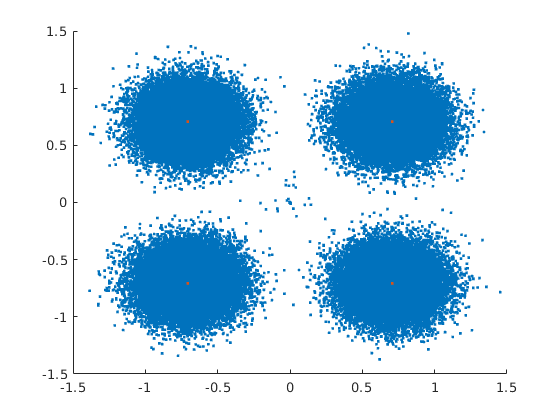
\includegraphics[scale=0.6]{plot-2v}

\section{Conclusion}
We managed to achieve all the results.

% that's all folks
\end{document}


